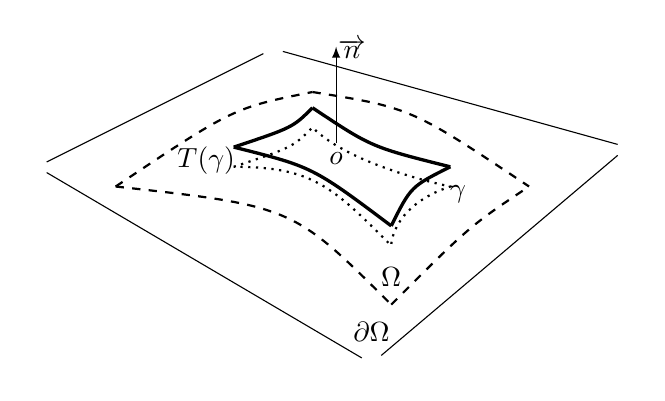
\begin{tikzpicture}[scale = 0.5]
\draw[dashed,thick] (-7.5,-1.5).. controls (-3,-2) and (-3,-2) .. (-0.5,-4.5);
\draw[dashed,thick](-0.5,-4.5) .. controls (1.5,-2.5) and (1.5,-2.5) .. (3,-1.5);
\draw[dashed,thick] (-7.5,-1.5) .. controls (-4.5,0.5) and (-4.5,0.5) .. (-2.5,0.9);
\draw[dashed,thick] (-2.5,0.9) .. controls (0,0.5) and (0,0.5) .. (3,-1.5);
\node (v1) at (-3.5,2) {};
\node (v4) at (-9.5,-1) {};
\node (v3) at (-1,-6) {};
\node (v2) at (5.5,-0.5) {};
\draw  (v1) edge (v2);
\draw  (v2) edge (v3);
\draw  (v3) edge (v4);
\draw  (v4) edge (v1);
\draw [dotted,thick](-4.5,-1) .. controls (-3,-0.5) and (-3,-0.5) .. (-2.5,0) .. controls (-1.5,-1) and (1,-1.5) .. (1,-1.5) .. controls (-0.5,-2) and (-0.5,-3) .. (-0.5,-3) .. controls (-2,-1.5) and (-2.5,-1) .. (-4.5,-1);
\node at (-2,-1) {};
\node (v5) at (-1.9,-0.8) {$o$};
%\draw[] at (-2,-1) ;
\draw[very thick] (-4.5,-0.5) .. controls (-2.5,-1) and (-2.5,-1) .. (-0.5,-2.5) ;
\draw[very thick]  (-0.5,-2.5) .. controls (0,-1.5) and (0,-1.5) .. (1,-1);
\draw [very thick] (1,-1) .. controls (-1,-0.5) and (-1,-0.5) .. (-2.5,0.5);
\draw  [very thick](-2.5,0.5) .. controls (-3,0) and (-3,0) .. (-4.5,-0.5);
\node at (-0.5,-3.8) {$\Omega$};
\node at (-1,-5.2) {$\partial \Omega$};
\node at (1.2,-1.7) {$ \gamma$};
\node at (-5.2,-0.83) {$ T(\gamma)$};
\node at (-2,-1) {};
\node (v6) at (-1.9,2.3) {};
\draw[-latex]  (v5) edge (v6);
\node at (-1.5,2) {$\overrightarrow{n}$};
\end{tikzpicture}